%%%%%%%%%%%%%%%%%%%%%%%%%%%%%%%%%%%%%%%%%
% Beamer Presentation
% LaTeX Template
% Version 1.0 (10/11/12)
%
% This template has been downloaded from:
% http://www.LaTeXTemplates.com
%
% License:
% CC BY-NC-SA 3.0 (http://creativecommons.org/licenses/by-nc-sa/3.0/)
%
%%%%%%%%%%%%%%%%%%%%%%%%%%%%%%%%%%%%%%%%%

%----------------------------------------------------------------------------------------
%	PACKAGES AND THEMES
%----------------------------------------------------------------------------------------

\documentclass{beamer}

\mode<presentation> {

% The Beamer class comes with a number of default slide themes
% which change the colors and layouts of slides. Below this is a list
% of all the themes, uncomment each in turn to see what they look like.

%\usetheme{default}
%\usetheme{AnnArbor}
%\usetheme{Antibes}
%\usetheme{Bergen}
%\usetheme{Berkeley}
%\usetheme{Berlin}
%\usetheme{Boadilla}
%\usetheme{CambridgeUS}
%\usetheme{Copenhagen}
%\usetheme{Darmstadt}
%\usetheme{Dresden}
%\usetheme{Frankfurt}
%\usetheme{Goettingen}
%\usetheme{Hannover}
%\usetheme{Ilmenau}
%\usetheme{JuanLesPins}
%\usetheme{Luebeck}
\usetheme{Madrid}
%\usetheme{Malmoe}
%\usetheme{Marburg}
%\usetheme{Montpellier}
%\usetheme{PaloAlto}
%\usetheme{Pittsburgh}
%\usetheme{Rochester}
%\usetheme{Singapore}
%\usetheme{Szeged}
%\usetheme{Warsaw}

% As well as themes, the Beamer class has a number of color themes
% for any slide theme. Uncomment each of these in turn to see how it
% changes the colors of your current slide theme.

%\usecolortheme{albatross}
%\usecolortheme{beaver}
%\usecolortheme{beetle}
%\usecolortheme{crane}
%\usecolortheme{dolphin}
%\usecolortheme{dove}
%\usecolortheme{fly}
%\usecolortheme{lily}
%\usecolortheme{orchid}
%\usecolortheme{rose}
%\usecolortheme{seagull}
%\usecolortheme{seahorse}
%\usecolortheme{whale}
%\usecolortheme{wolverine}

%\setbeamertemplate{footline} % To remove the footer line in all slides uncomment this line
%\setbeamertemplate{footline}[page number] % To replace the footer line in all slides with a simple slide count uncomment this line

%\setbeamertemplate{navigation symbols}{} % To remove the navigation symbols from the bottom of all slides uncomment this line
}

\usepackage{graphicx} % Allows including images
\usepackage{booktabs} % Allows the use of \toprule, \midrule and \bottomrule in tables
\usepackage{listings}
\usepackage{amsmath}
\usepackage{algpseudocode,algorithm,algorithmicx}

\lstdefinestyle{customjava}{
  breaklines=true,
  frame=L,
  xleftmargin=\parindent,
  language=Java,
  showstringspaces=false,
  basicstyle=\footnotesize\ttfamily,
  keywordstyle=\bfseries\color{green!40!black},
  commentstyle=\itshape\color{gray!40!black},
  identifierstyle=\color{blue},
  stringstyle=\color{orange},
}

\lstdefinestyle{customcpp}{
  breaklines=true,
  frame=L,
  xleftmargin=\parindent,
  language=C++,
  showstringspaces=false,
  basicstyle=\footnotesize\ttfamily,
  keywordstyle=\bfseries\color{green!40!black},
  commentstyle=\itshape\color{gray!40!black},
  identifierstyle=\color{blue},
  stringstyle=\color{orange},
}
%----------------------------------------------------------------------------------------
%	TITLE PAGE
%----------------------------------------------------------------------------------------

\title[Disk Systems]{Disk Systems} % The short title appears at the bottom of every slide, the full title is only on the title page

\author{Jonathan Windle} % Your name
\institute[UEA] % Your institution as it will appear on the bottom of every slide, may be shorthand to save space
{
University of East Anglia \\ % Your institution for the title page
\medskip
\textit{J.Windle@uea.ac.uk} % Your email address
}
\date{\today} % Date, can be changed to a custom date

\begin{document}

\begin{frame}
\titlepage % Print the title page as the first slide
\end{frame}

\begin{frame}[allowframebreaks]
\frametitle{Overview} % Table of contents slide, comment this block out to remove it
\tableofcontents % Throughout your presentation, if you choose to use \section{} and \subsection{} commands, these will automatically be printed on this slide as an overview of your presentation
\end{frame}

%-------------------------------------------------------------------
\section{Secondary Storage}
\begin{frame}
\frametitle{Secondary Storage}
\begin{itemize}
\item Most secondary storage devices utilise magnetic media
\item A read-write head is moved across the media
\item Early tape systems accessed data sequentially, data is streamed in order from first bit to last sequential bit, access not practical for interactive systems
\item More modern devices use magnetic disks, data can be accessed in any order (random access)
\item Early magnetic disk system used large removable disks (platters)
\item Over time these have gotten progressively smaller
\item Floppy Disk removable storage media now largely replaced by semiconductor memory
\end{itemize}
\end{frame}
%------------------------------------------------------------------
\section{Hard Drives}
\begin{frame}
\frametitle{Hard Drives}
\begin{itemize}
\item Platters are formaed from billions of ferrite grains
\item Limiting factors affecting actual storage density:
\begin{itemize}
\item Interference at boundaries betwen logic 0 and 1 (opposing magnetic domains)
\item Heat.
\end{itemize}
\end{itemize}
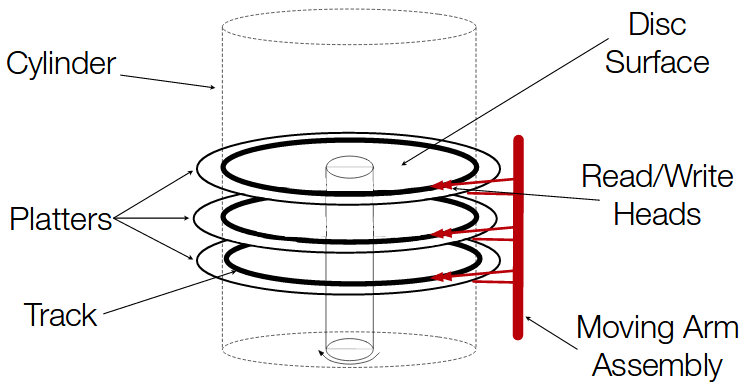
\includegraphics[scale=0.2]{hdd.png}
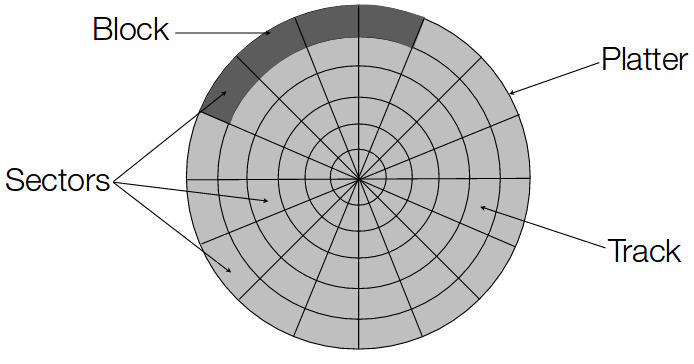
\includegraphics[scale=0.2]{disk.png}
\end{frame}
%-----------------------------------------------------------------
\subsection{Issues}
\begin{frame}
\frametitle{Issues}
\begin{itemize}
\item Main (semiconductor) memory provides almost uniform access time
\item Can read/write any location equally quickly
\item But access time for disk store depends on position of bits on actual disk relative to read/write head
\begin{itemize}
\item Requires mechanical movements
\item Relavent regions of disc must be located
\item Aim to minimise amount of time spent searching
\end{itemize}
\end{itemize}
\end{frame}
%------------------------------------------------------------------
\subsection{Typical Disk Access Operations}
\begin{frame}
\frametitle{Typical Disk Access Operations}
\begin{itemize}
\item OS specifies location of the data (head/cylinder/sector)
\item Moving arm assembly moves disk arm to cylinder
\item Time takken to move known as seek time
\item Disk must be rotated until sector is under read/write head
\item Time delay referred to ass rotational latency
\item Data is read/written as sector moves past head
\item Referred to as transmission time
\end{itemize}
\end{frame}
%------------------------------------------------------------------
\subsection{Read-Write Latency}
\begin{frame}
\frametitle{Read-Write Latency}
\begin{itemize}
\item Disk access time is a  function of the three delays
\begin{itemize}
\item Seek time + rotational latency + transmission time
\item These all vary depending on the relative position of the read-write head and sector of interest.
\end{itemize}
\item Typically in the order of milliseconds
\item In this time the CPU may have executed millions of instructions 
\item Many processes are becoming increasingly I/O bound:
\begin{itemize}
\item CPU/Memory speeds are increasing rapidly (due to advances in semiconductor fabrication) while disk access has not increased proportionally.
\end{itemize}
\end{itemize}
\end{frame}
%-------------------------------------------------------------------
\section{Disk Scheduling}
\begin{frame}
\frametitle{Disk Scheduling}
\begin{itemize}
\item Disk access requires scheduling:
\begin{itemize}
\item Many processes can request disk access much faster than they can be serviced
\item Both absolute and relative locations of data are important. CPU/memory speeds are increasing rapidly, disk access has not.
\end{itemize}
\item Scheduling disk access imposes additional delay.
\item For examples, assume cylinder requests are in order:
\begin{itemize}
\item 33,72,47,8,99,74,42,75
\end{itemize}
\item Assume read-write head is initially positioned at cylinder 63:

\end{itemize}
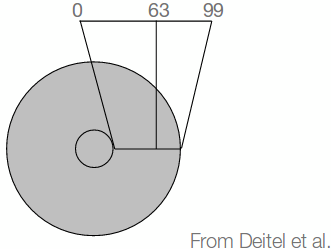
\includegraphics[scale=0.35]{cyl.png}
\end{frame}

%-----------------------------------------------------------------
\subsection{First come first served}
\begin{frame}
\frametitle{First come first served}
\begin{itemize}
\item Requests are serviced in order they come.
\item A fair policy
\item Results in long waiting times if load is high
\item Tendancy to switch between tracks/sectors
\end{itemize}
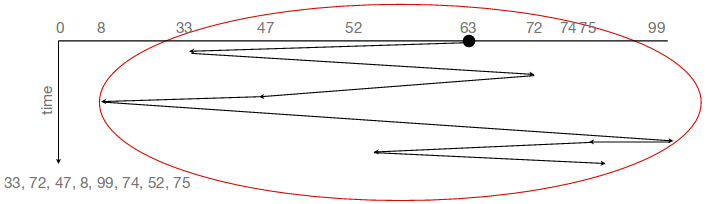
\includegraphics[scale=0.35]{fcfs.png}
\end{frame}
%-----------------------------------------------------------------
\subsection{Shortest-seek-time-first}
\begin{frame}
\frametitle{Shortest-seek-time-first}
\begin{itemize}
\item Schedule request closest to current location of r/w head
\item Achieves high throughput
\item Does not ensure fairness
\item Relatively high variance in response time
\end{itemize}
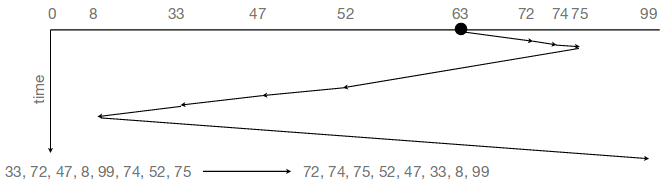
\includegraphics[scale=0.35]{sstf.png}
\end{frame}

%------------------------------------------------------------------
\subsection{Elevator Algorithm (SCAN)}
\begin{frame}
\frametitle{Elevator Algorithm (SCAN)}
\begin{itemize}
\item Choose shortesk seek time in preferred direction
\begin{itemize}
\item At inner/outer cylinder switch direction
\end{itemize}
\item Offers high throughpput, low mean response time, and lower variance of response time
\item Could suffer indefinite postponement (but unlikely)
\item Bias towards middle cylinders
\item Unnecessary seek operations are performed to scan to the inner/outer most cylinder
\end{itemize}
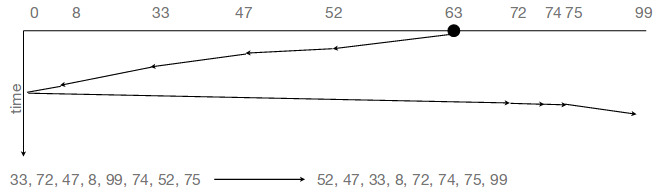
\includegraphics[scale=0.35]{scan.png}
\end{frame}
%------------------------------------------------------------------
\subsection{Circular-SCAN (C-SCAN)}
\begin{frame}
\frametitle{Circular-SCAN (C-SCAN)}
\begin{itemize}
\item Modification of SCAN strategy
\item Choose shortest seek time in inward direction
\begin{itemize}
\item At inner most cylinder, jump back to outermost
\end{itemize}
\item Further reduces variance of response time
\item Removes bias towards middle cylinders
\item Performs unnecessary seek operations
\item Could suffer from indefinite postponement (but unlikely)
\end{itemize}
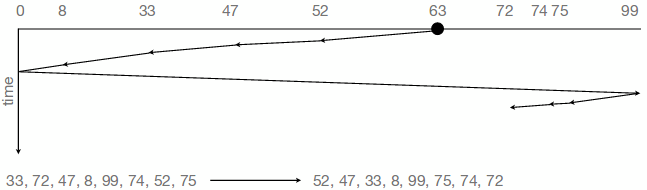
\includegraphics[scale=0.35]{CSCAN.png}
\end{frame}
%------------------------------------------------------------------
\subsection{Freeze-SCAN (F-SCAN)}
\begin{frame}
\frametitle{Freeze-SCAN (F-SCAN)}
\begin{itemize}
\item Modification of SCAN
\item Choose shortest seek time in inwards direction
\begin{itemize}
\item Service only requests present at the beginning of sweeep
\item Order incoming requests during sweet for optimum service
\item Process waiting requests on return
\end{itemize}
\item Solves problem of indefinite postponement
\end{itemize}
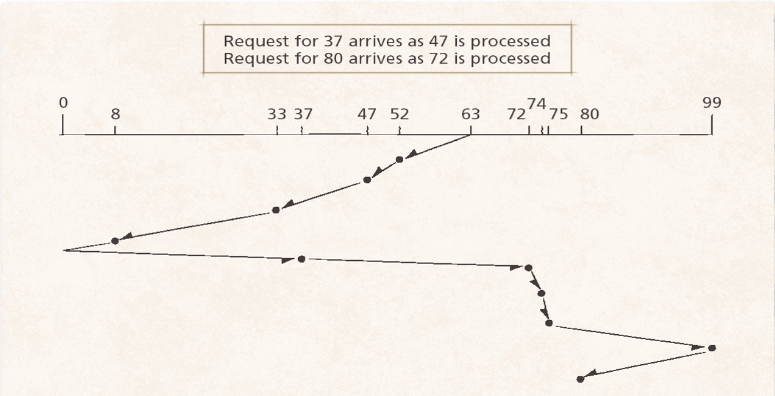
\includegraphics[scale=0.35]{fscan.png}
\end{frame}
%------------------------------------------------------------------
\subsection{Where its performed}
\begin{frame}
\frametitle{Where it's performed}
\begin{itemize}
\item The OS could filter requests before sending to the disk controller.
\begin{itemize}
\item OS has knowledge of the overall system load requirements
\end{itemize}
\item Disk controllers themselves are becoming increasingly intelligent
\begin{itemize}
\item Takes burden off OS
\end{itemize}
\item Likely that both perform scheduling
\end{itemize}
\end{frame}
%--------------------------------------------------------------------
\subsection{Other performance factors}
\begin{frame}
\frametitle{Other performance factors}
\begin{itemize}
\item Better placement of files on disk:
\begin{itemize}
\item Ensure disk is defragmented to minimise seek time
\item Scheduling overhead can degrade performance
\item Consider transferring blocks rather than sectors
\end{itemize}
\item Utilise data compression/decompression
\begin{itemize}
\item Less data needs read/written for same information storage
\item Assume decompression time is less than inflated read/write time
\end{itemize}
\item Use disk cache buffer
\begin{itemize}
\item Memory to store data to be written
\item Only write during periods of relatively light load
\item Give preference to read operations
\item Need to worry about consistency
\end{itemize}
\item Store multiple copies of frequently accessed data:
\begin{itemize}
\item Read from copythat is closes to r/w head
\item Need to worry about consistency
\item Reduces effective disk capacity
\end{itemize}
\item Utilise RAID (Redundant Array of Independent Disks)
\begin{itemize}
\item Data stored on multiple drives for fast access.
\end{itemize}
\end{itemize}
\end{frame}
%------------------------------------------------------------------
\section{Summary}
\begin{frame}
\frametitle{Summary}
\begin{itemize}
\item Disk access is slow (several milliseconds)
\begin{itemize}
\item Function of 3 effective delays
\end{itemize}
\item Physical layout of bits on drive are addresses as:
\begin{itemize}
\item Surface
\item Cylinder
\item Sector
\end{itemize}
\item OS works at block level
\begin{itemize}
\item Typically many sectors per block
\end{itemize}
\end{itemize}
\end{frame}
%------------------------------------------------------------------

\begin{frame} 
\Huge{\centerline{The End}}
\end{frame}

\end{document}